% Paquets généraux
\documentclass[a4paper,12pt,titlepage,twoside]{article}
\usepackage[T1]{fontenc}
\usepackage[utf8]{inputenc}
\usepackage[french]{babel}
\usepackage{subcaption}
\addto\captionsfrench{%
  \renewcommand{\tablename}{Tableau}%
}
\usepackage[gen]{eurosym}
%\usepackage[dvips]{graphicx}
\usepackage{minted}
\usepackage{fancyhdr}
\usepackage{pdfpages} 
\usepackage{multido}
\usepackage{hyperref}
\usepackage{textcomp}
\usepackage{schemabloc}
%\usepackage[bitstream-charter]{mathdesign}
\usepackage{array}
\newcolumntype{P}[1]{>{\centering\arraybackslash}p{#1}}
\usepackage[shortlabels]{enumitem}
\usepackage[framemethod=TikZ]{mdframed}
\usepackage{algpseudocode}
\usepackage{algorithm}

\newcommand{\nom}{Porte coulissante de magasin}
\newcommand{\numero}{01}
\newcommand{\sujet}{Porte coulissante}
\newcommand{\jour}{Samedi 26 septembre 2026}
\newcommand{\auteurun}{Renaud Costadoat}
\newcommand{\auteurdeux}{Françoise Puig}

%\usepackage{style}
\usepackage{bodegraph}
%\usepackage{rpcinematik}
\usepackage[locale = FR]{siunitx}
\usepackage{caption}
\newcommand{\institute}{Lycée Dorian}
\usepackage{calc}

\usepackage{listings}
\usepackage{fancyvrb}
\usepackage{color}
\usepackage{xcolor}
\usepackage{colortbl}
\usepackage{helvet}
\usepackage[frenchmath]{newtxsf} % for sans serif symbols
\renewcommand{\familydefault}{\sfdefault}
%\usepackage{amsfonts}
%\usepackage{amsmath}
%\usepackage{lmodern}
\usepackage{mathastext}
%\usepackage{xspace}
\usepackage{varioref}
\usepackage{tabularx}
%\usepackage{floatflt}
\usepackage{graphics}
\usepackage{wrapfig}
\usepackage{textcomp}
\usepackage{tikz,tkz-tab}
\usepackage[european resistor, european voltage, european current]{circuitikz}
\usepackage{wrapfig}
\usepackage{gensymb}
\usepackage[percent]{overpic}
\usetikzlibrary{babel}
\usepackage{ifthen}
\usepackage{cancel}
\usepackage{etoolbox}
\usepackage{multirow}
%\usepackage{boxedminipage}
\definecolor{gris25}{gray}{0.75}
\definecolor{bleu}{RGB}{18,33,98}
\definecolor{bleuf}{RGB}{42,94,171}
\definecolor{bleuc}{RGB}{231,239,247}
\definecolor{bleum}{RGB}{160,195,226}
\definecolor{rougef}{RGB}{185,18,27}
\definecolor{rougec}{RGB}{255,188,204}%255,230,231
\definecolor{vertf}{RGB}{103,126,82}
\definecolor{vertc}{RGB}{220,255,191}
\definecolor{forestgreen}{rgb}{0.13,0.54,0.13}
\definecolor{blcr}{rgb}{0.59,0.69,0.84}
\definecolor{blfr}{rgb}{0.32,0.51,0.75}
\definecolor{orfr}{rgb}{0.90,0.42,0.15}
\definecolor{orcr}{rgb}{0.90,0.65,0.50}
\definecolor{orangef}{rgb}{0.659,0.269,0.072}
\definecolor{orange}{rgb}{0.58,0.35,0.063}
\definecolor{orangec}{rgb}{0.43,0.32,0.25}
\definecolor{rcorrect}{rgb}{0.6,0,0}
\definecolor{sequence}{rgb}{0.75,0.75,0.75}
\definecolor{competences}{rgb}{0.61,0.73,0.35}
\definecolor{rose}{HTML}{ff00ff}
\definecolor{grisf}{HTML}{222222}
\definecolor{grisc}{HTML}{636363}
\definecolor{normal}{HTML}{4087c4}
\definecolor{info}{HTML}{5bc0de}
\definecolor{success}{RGB}{92,184,92}
\definecolor{warning}{RGB}{240,173,78}
\definecolor{danger}{RGB}{217,83,79}
\hypersetup{                    % parametrage des hyperliens
    colorlinks=true,                % colorise les liens
    breaklinks=true,                % permet les retours à la ligne pour les liens trop longs
    urlcolor= blfr,                 % couleur des hyperliens
    linkcolor= orange,                % couleur des liens internes aux documents (index, figures, tableaux, equations,...)
    citecolor= forestgreen                % couleur des liens vers les references bibliographiques
    }

\newcolumntype{M}[1]{>{\centering\arraybackslash}m{#1}}
\definecolor{codegreen}{rgb}{0,0.6,0}
\definecolor{codegray}{rgb}{0.5,0.5,0.5}
\definecolor{codepurple}{rgb}{0.58,0,0.82}
\definecolor{backcolour}{rgb}{0.95,0.95,0.92}

\lstdefinestyle{mystyle}{
    backgroundcolor=\color{backcolour},   
    commentstyle=\color{codegreen},
    keywordstyle=\color{magenta},
    numberstyle=\tiny\color{codegray},
    stringstyle=\color{codepurple},
    basicstyle=\ttfamily\footnotesize,
    breakatwhitespace=false,         
    breaklines=true,                 
    captionpos=b,                    
    keepspaces=true,                 
    numbers=left,                    
    numbersep=5pt,                  
    showspaces=false,                
    showstringspaces=false,
    showtabs=false,                  
    tabsize=2
}

\lstset{style=mystyle}

% Mise en page
\pagestyle{fancy}

\setlength{\hoffset}{-18pt}
\setlength{\oddsidemargin}{0pt} 	% Marge gauche sur pages impaire2s
\setlength{\evensidemargin}{0pt} 	% Marge gauche sur pages paires
\setlength{\marginparwidth}{00pt} 	% Largeur de note dans la marge
\setlength{\headwidth}{481pt} 	 	% Largeur de la zone de tête (17cm)
\setlength{\textwidth}{481pt} 	 	% Largeu\textbf{r de la zone de texte (17cm)
\setlength{\voffset}{-18pt} 		% Bon pour DOS
\setlength{\marginparsep}{7pt}	 	% Séparation de la marge
\setlength{\topmargin}{-30pt} 		% Pas de marge en haut
\setlength{\headheight}{55pt} 		% Haut de page
\setlength{\headsep}{20pt} 		% Entre le haut de page et le texte
\setlength{\footskip}{30pt} 		% Bas de\textbf{ page + séparation
\setlength{\textheight}{700pt} 		% Hauteur de l'icone zone de texte (25cm)
\setlength\fboxrule{1 pt}
\renewcommand{\baselinestretch}{1}
\setcounter{tocdepth}{1}
\newcommand{\cadre}[2]
{\fbox{
  \begin{minipage}{#1\linewidth}
   \begin{center}
    #2\\
   \end{center}
  \end{minipage}
 }
}

\newcommand{\repon}[1]
{
~\ \\
\begin{tabular}{|m{\linewidth}|}
 \hline
\multido{}{#1}{\\ \hline}
\end{tabular}
}


\newcommand{\objectif}[1]{
\mdfsetup{%
frametitle={%
\tikz[baseline=(current bounding box.east),outer sep=0pt]
\node[anchor=east,rectangle,fill=bleum]
{\strut Objectif~};}}
\mdfsetup{innertopmargin=10pt,linecolor=bleum,%
linewidth=2pt,topline=true,%
frametitleaboveskip=\dimexpr-\ht\strutbox\relax
}
\begin{mdframed}[]\relax%
#1
\end{mdframed}}


\newcounter{num_quest} \setcounter{num_quest}{0}
\newcounter{num_rep} \setcounter{num_rep}{0}
\newcounter{num_cor} \setcounter{num_cor}{0}

\newcommand{\feuilleDR}[1]{
	\begin{tikzpicture}
		\draw[gray!30](0,0)grid[step=0.5cm](\linewidth,#1);
	\end{tikzpicture}
}

%\newcommand{\question}[1]{\refstepcounter{num_quest}\par
%~\ \\ \parbox[t][][t]{0.15\linewidth}{\textbf{Question \arabic{num_quest}}}\parbox[t][][t]{0.85\linewidth}{#1\label{q\the\value{num_quest}}}\par
%}

\newcommand{\question}[1]{\refstepcounter{num_quest}\par
~\ \\ \textbf{Question \arabic{num_quest} : }#1\label{q\the\value{num_quest}}\par
}

\newcommand{\posetafigure}[3]{
\begin{figure}[ht!]
 \begin{center}
  \includegraphics[width=#2\linewidth]{img/#1}
 \end{center}
 \caption{\label{#1} #3}
\end{figure}}

\newcommand{\goforum}{
\begin{figure}

\end{figure}
\begin{center}
 
\includegraphics[width=0.7\linewidth]{../../../img/go_forum}
\end{center}
\label{go_forum}
\caption{J'pète les plombs}
\end{figure}}

\newcommand{\reponse}[4][1]
{\noindent
\parbox{\textwidth}{
\rule{\linewidth}{.5pt}\\
\textbf{Question\ifthenelse{#1>1}{s}{} \multido{}{#1}{%
\refstepcounter{num_rep}\ref{q\the\value{num_rep}} }:} ~\ \\
\ifdef{\public}{#3 \ifthenelse{#2>0}{~\ \\ 	\feuilleDR{#2}}}{#4}
}}

\NewDocumentEnvironment{reponseminted}{O{1} m m +b}{%
% ======== BEGIN ========
\noindent
\begin{minipage}{\textwidth}
\rule{\linewidth}{.5pt}\\
\textbf{Question%
\ifthenelse{#1>1}{s}{}%
\multido{}{#1}{\refstepcounter{num_rep}\ref{q\the\value{num_rep}}}:}%
\\[0.4em]

\ifdef{\public}{%
    #3%
    \ifthenelse{#2>0}{\\[0.5em]\feuilleDR{#2}}{}%
}{}

\end{minipage}

% ======== END OF MINIPAGE ========

\ifdef{\public}{}{% si pas public, afficher le corrigé verbatim
#4%
}
}



\newboolean{printdr}
\newboolean{printcor}
\setboolean{printdr}{false}
\setboolean{printcor}{false}

\newcommand{\reponseinfo}[2][1]
{\noindent
\rule{\linewidth}{.5pt}\\
\textbf{Question\ifthenelse{#1>1}{s}{} \multido{}{#1}{%
\refstepcounter{num_rep}\ref{q\the\value{num_rep}} }:} ~\ \\
\ifdef{\public}{\parbox{\textwidth}{\ifthenelse{#2>0}{~\ \\ 	\feuilleDR{#2}}}
\setboolean{printdr}{true}\setboolean{printcor}{false}}
{\setboolean{printdr}{false}\setboolean{printcor}{true}}
}

\newcommand\sautpage[1]{
\ifdef{\public}{\multido{}{#1}{~\ \newpage}}
}


\makeatletter
\newcommand\modulo[2]{
    \newcounter{lastpagesujet}
	\setcounter{lastpagesujet}{#1}
    \divide\value{lastpagesujet} by #2
    \multiply\value{lastpagesujet} by #2
    \advance\value{lastpagesujet} by #2
    \advance\value{lastpagesujet} by 1\relax
    }
\makeatother

\newcommand{\finsujet}[1]
{
    \begin{center}
    \Large{FIN}
    \end{center}
        
    \ifthenelse{\equal{#1}{public}}{\def\public{}}{}

}

\newcommand{\debutcor}
{	
    \ifdef{\public}{
        \pagestyle{docreponse}
	}{\pagestyle{correction}}


    \ifdef{\public}{
    \begin{center}
        \begin{tikzpicture} 
            \draw (0,0) rectangle (2,2);
            \draw (0,0) -- (2,2);
            \draw (1.5,0.5) node {\large 20};
            \draw (2,0) rectangle (17,2);
            \draw (4,1.7) node {\large Commentaires:};
            \draw (0,2) rectangle (8.5,3);
            \draw (8.5,2) rectangle (17,3);
            \draw (1,2.5) node {\large NOM:};
            \draw (9.7,2.5) node {\large Prénom:};
        \end{tikzpicture}
    \end{center}
    }
}

\newcommand{\ecrirenom}
{	

    \ifdef{\public}{
    \newpage
    
    \begin{center}
        \begin{tikzpicture} 
            \draw (0,0) rectangle (8.5,1);
            \draw (8.5,0) rectangle (17,1);
            \draw (1,0.5) node {\large NOM:};
            \draw (9.7,0.5) node {\large Prénom:};
        \end{tikzpicture}
    \end{center}
    
    }
}

%\newcommand{\repcarre}[2]
%{
%~\ \\
%\begin{tikzpicture}
%\draw [fill=white] (0,0) rectangle +(\linewidth,#1);
%\node[align=left] at (1.1,#2-0.3) {\textbf{Question #1:}};
%\end{tikzpicture}
%}

\newcommand{\titre}[1]
{\begin{center}
\cadre{0.8}{\huge #1} 
\end{center}
}


%Définition des torseurs :
\newcommand{\torseur}[2]{\left\{\mathcal{#1}_{#2} \right\}}
\newcommand{\torseurh}[3]{\left\{\genfrac{}{}{0pt}{0}{#1}{#2}\right\}_{#3}}
\newcommand{\torseurv}[8]{\left\{
\begin{matrix}
#1 & #4 \\ #2 & #5 \\ #3 &#6
\end{matrix}
\right\}_{{#7},{#8}}}

%Définition des torseurs :
%\newcommand{\torseur}[2]{\left \{\mbox{\relsize{2}{$\mathcal {#1}$}\relsize{-2}}\phantom{}_{\mbox{\scriptsize $#2$}} \right \}}
%\newcommand{\torseurh}[3]{\left\{\genfrac{}{}{0pt}{0}{#1}{#2}\right\}_{#3}}
%\newcommand{\torseurv}[8]{
%\left\{\begin{array}{@{}c|c@{}} #1 & #4 \\ #2 & #5 \\ #3 & #6 \end{array} \right\}_{#7,#8}
%}
\newcommand{\derivee}[2]{\left.\dfrac{\d #1}{\d t}\right|_{#2}}
\newcommand{\tripleint}{\int\!\!\!\!\!\int\!\!\!\!\!\int}

% Notation cinématique et statique
\newcommand{\cinematique}[2]{\mbox{#1}/\mbox{#2}}
\newcommand{\statique}[2]{\mbox{#1}\rightarrow\mbox{#2}}
\newcommand{\moment}[3]{\vv {#1}_{\scriptsize{#3}}(#2)}
\newcommand{\resultante}[2]{\vv {#1}_{\scriptsize{#2}}}


%Commande de base
\newcommand{\jo}{\left(j\omega\right)} % j \omega dans l'analyse fréquentielle
\newcommand{\tl}{\xrightarrow{\mathcal{L}}} % transformée de laplace sur fleche
\newcommand{\tli}{\xrightarrow{\mathcal{L}^{-1}}} % transformée inverse de laplace sur fleche
\renewcommand{\d}[1][]{\mathrm{d#1}}
\newcommand{\dd}[1][]{\mathrm{d#1}}
\newcommand{\vect}[2]{{#1}\wedge{#2}}
\newcommand{\base}[3]{(\vec #1,\vec #2,\vec #3)}
\newcommand{\vectbase}[4]{{\vphantom{\left| \begin{matrix}
#1\\#2\\#3 \end{matrix} \right|}}_{#4}{\left| \begin{matrix}
#1\\#2\\#3 \end{matrix} \right.}}
%Pour avoir les paragraphes sous la forme I, II, III
\renewcommand{\thesection}{\Roman{section}}
\setcounter{secnumdepth}{3}
\renewcommand{\Frlabelitemii}{$\bullet$}

% En tête et pied de page
\lhead{\nom}
\rhead{
\includegraphics[width=2cm]{../../../img/logo}}
\lfoot{\auteurun,\ \auteurdeux}
\cfoot{Page \thepage}

\fancypagestyle{docreponse}{%
  \fancyhf{}
%  \fancyhead[LO]{NOM Prénom: .............................}
  \rhead{
\includegraphics[width=2cm]{../../../img/logo}\hspace{2pt}}
  \ifdef{\auteurdeux}{\lfoot{\auteurun,\ \auteurdeux}}{\lfoot{\auteurun}}
  \rfoot{\sujet}
  \lfoot{Document réponse}
  \cfoot{Page \thepage}
   }

\fancypagestyle{correction}{%
  \fancyhf{}
  \lhead{\colorbox{danger}{\begin{minipage}{0.65\paperwidth} \textcolor{white}{\textbf{Correction}} \end{minipage}} }
  \rhead{
\includegraphics[width=2cm]{../../../img/logo}}
  \lfoot{Renaud Costadoat, Françoise Puig}
  \rfoot{\colorbox{danger}{\begin{minipage}{0.3\paperwidth} \begin{flushright}\textcolor{white}{\textbf{Correction}}\end{flushright} \end{minipage}} }
  \cfoot{Page \thepage}
}

\fancypagestyle{correctioninfo}{%
  \fancyhf{}
  \lhead{\colorbox{danger}{\begin{minipage}{0.65\paperwidth} \textcolor{white}{\textbf{Correction}} \end{minipage}} }
  \rhead{
\includegraphics[width=2cm]{../../../img/logo}}
  \lfoot{Renaud Costadoat, Juliette Genzmer}
  \rfoot{\colorbox{danger}{\begin{minipage}{0.6\paperwidth} \begin{flushright}\textcolor{white}{\textbf{Correction}}\end{flushright} \end{minipage}} }}

\renewcommand{\footrulewidth}{0.4pt}

\usepackage{eso-pic}
\newcommand{\BackgroundPic}{%
\put(0,0){%
\parbox[b][\paperheight]{\paperwidth}{%
\vfill
\begin{center}
\hspace{0.5cm}\vspace{0.5cm}

\includegraphics[width=\paperwidth,height=\paperheight,%
keepaspectratio]{../../../img/fond3}%
\end{center}
\vfill
}}}

\newcommand{\BackgroundPicdeux}{%
\put(25,-30){%
\parbox[b][\paperheight]{\paperwidth}{%
\vfill
\begin{center}
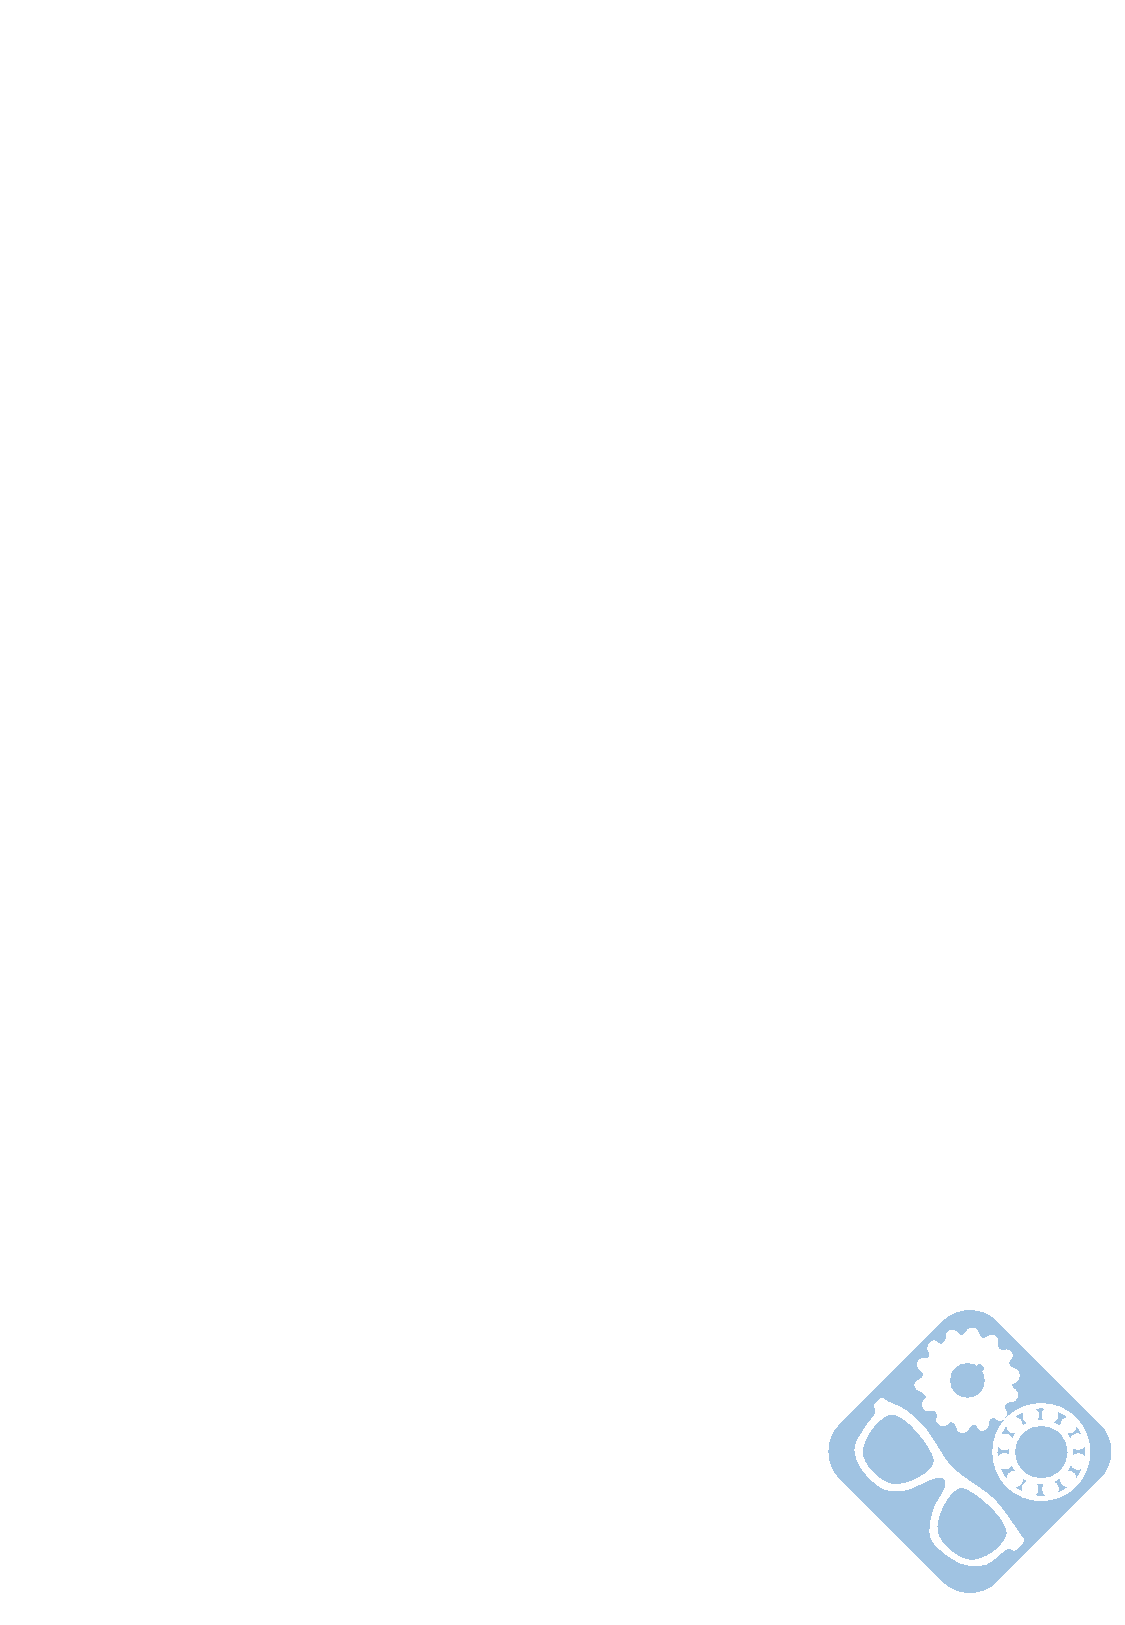
\includegraphics[width=\paperwidth,height=\paperheight,%
keepaspectratio]{../../../img/fond4}%
\end{center}
\vfill
}}}

\begin{document}

\pagestyle{empty}

\AddToShipoutPicture*{\BackgroundPic}


\includegraphics[width=2cm]{../../../img/logo}

\Huge{DS \numero - \sujet}

\vspace{1cm}

\ifdef{\prive}{\begin{center}\colorbox{danger}{\Huge{Avec Correction}}\end{center}}{}

\begin{center}
\centering\huge{PTSI}
\end{center}

\vspace{2cm}


\begin{center}
\centering\Large{\jour}
\end{center}

\vspace{2cm}

\normalsize

\tableofcontents

\newpage

\AddToShipoutPicture{\BackgroundPicdeux}

\pagestyle{fancy}

\begin{center}
\Huge \sujet
\end{center}


\normalsize



\section{Mise en situation}

On étudie l'entraînement d'une porte coulissante automatique de magasin. Le mouvement de translation du vantail est assuré par un moteur à courant continu, entraînant une poulie de rayon $r$ sur laquelle est fixée une courroie solidaire de la porte.

\begin{figure}
\begin{center}
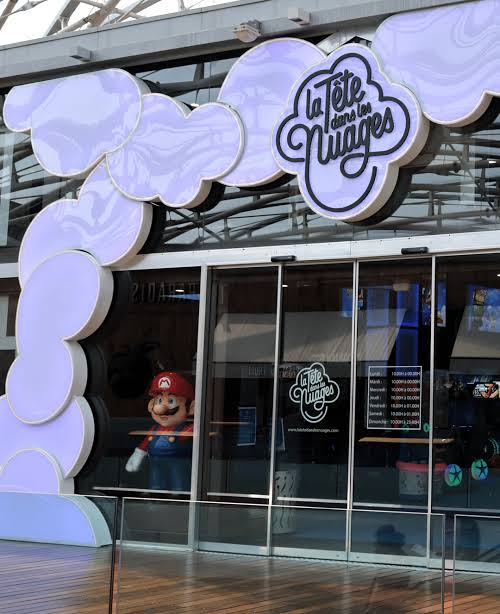
\includegraphics[width=0.5\linewidth]{img/fig01.jpg}
\caption{\label{fig01}Portes coulissantes}
\end{center}
\end{figure}

\subsection{Équation électrique de l'induit}

En notant $v(t)$ la tension appliquée aux bornes de l'induit, $i(t)$ le courant d'induit, $R$ la résistance d'induit, $L$ son inductance, et $e(t) = K_e\cdot\omega(t)$ la force contre-électromotrice ($\omega(t)$ étant la vitesse angulaire du rotor), la loi des mailles donne :

\begin{equation}
L\cdot\frac{di(t)}{dt} + R\cdot i(t) = v(t) - K_e\cdot\omega(t)
\label{eq:elec}
\end{equation}

\subsection*{Équation mécanique}

Le couple électromagnétique développé par le moteur est $C_m(t) = K_t\cdot i(t)$. En appliquant le principe fondamental de la dynamique en rotation à l'ensemble \{rotor + réducteur + porte ramenée côté moteur\}, d'inertie totale $J$ et soumis à un frottement visqueux équivalent $b$, on obtient :

\begin{equation}
J\cdot\frac{d\omega(t)}{dt} + b\cdot\omega(t) = K_t\cdot i(t)
\label{eq:meca}
\end{equation}

\subsection*{Notations et valeurs numériques}

\begin{center}
\begin{tabular}{|c|l|c|}
\hline
\textbf{Symbole} & \textbf{Grandeur} & \textbf{Valeur} \\
\hline
$V_0$ & Tension d'alimentation (échelon) & $24\ V$ \\
$R$ & Résistance d'induit & $2\ \Omega$ \\
$L$ & Inductance d'induit & $5\cdot 10^{-5}\ H$ \\
$K_e$ & Constante de force contre-électromotrice & $0.05\ V\cdot s\cdot rad^{-1}$ \\
$K_t$ & Constante de couple & $0.05\ N\cdot m\cdot A^{-1}$ \\
$J$ & Inertie totale ramenée côté moteur & $0.000325\ kg\cdot m^2$ \\
$b$ & Frottement visqueux ramené au moteur & $0.02\ N\cdot m \cdot s\cdot rad^{-1}$ \\
$r$ & Rayon de la poulie d'entraînement & $0.02\ m$ \\
\hline
\end{tabular}
\end{center}

On suppose le système initialement au repos : $i(0) = 0$ et $\omega(0) = 0$. À l'instant $t=0$, on applique un échelon de tension $v(t) = V_0\cdot u(t)$, où $u(t)$ est l'échelon unité.

\section{Passage dans le domaine de Laplace}

\question{Les conditions initiales étant nulles, transformer les équations \eqref{eq:elec} et \eqref{eq:meca} dans le domaine de Laplace. On notera $V(p)$, $I(p)$ et $\Omega(p)$ les transformées de Laplace respectives de $v(t)$, $i(t)$ et $\omega(t)$.}

\vspace{0.5cm}

\question{À partir des deux équations précédentes, établir la fonction de transfert du système sous la forme canonique:

\[
H(p) = \frac{\Omega(p)}{V(p)}
\].}

\vspace{0.5cm}

\question{Identifier les paramètres $K$, $\omega_0$ et $\xi$ de la fonction de transfert.}

\vspace{0.5cm}

\question{À l'aide des données du tableau, calculer les valeurs numériques de $K$, $\omega_0$ et $\xi$.}

\question{Justifier alors que la fonction de transfert puisse s'écrire 
\[
H(p) = \frac{K}{1 + \tau p}
\]
Déterminer alors les valeurs numériques de $K$ et $\tau$.
}

\section{Réponse temporelle}

Un échelon de tension $v(t)=V_0$ est appliqué aux bornes du moteur.

\question{Déterminer $\omega_{+\infty}=\lim\limits_{t\rightarrow +\infty}\omega(t)$.}

\vspace{0.5cm}

\question{A quel tracé de la figure \ref{fig02} correspond $\omega(t)$ pour }

\begin{figure}
\begin{center}
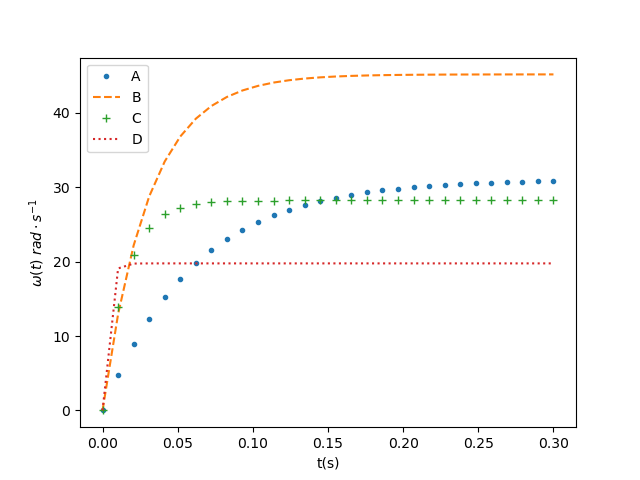
\includegraphics[width=\linewidth]{img/fig02}
\caption{\label{fig02}Tracé de réponses temporelles}
\end{center}
\end{figure}

\question{Quel est le temps de réponse à 5\% du système d'ouverture/fermeture de porte ?}

On note $v_p(t)$ la vitesse de translation de la porte.

\question{Justifier que l'on peut écrire $v_p(t)=r\cdot \omega(t)$}

\question{En déduire $v_{p+\infty}=\lim\limits_{t\rightarrow +\infty}v_p(t)$.}

Le temps de réponse étant considéré faible par rapport au temps de déplacement total de la porte, il sera supposé pour la suite que la porte s'ouvre à une vitesse constante $v_p(t)=v_{p+\infty}$. 

\question{En combien de temps la porte parcours-t-elle les 1.2m de sa course ?}

\section{Questions de cours}

Soit la fonction de transfert suivante:
\[H_2(p)=\dfrac{K}{1+\dfrac{2\cdot\xi}{\omega_0}\cdot p+\dfrac{p^2}{\omega_0^2}},\ avec\ \xi>1\].

\question{Déterminer l'expression des pôles de cette fonction de transfert en fonction de $\xi$ et de $\omega_0$.}

\vspace{1cm}

Soit la fonction de transfert suivante:
\[H_3(p)=\dfrac{S_3(p)}{E_3(p)}=\dfrac{8}{1+0.3\cdot p+0,02\cdot p^2}\].


\question{Montrer qu'elle peut s'écrire sous la forme suivante en déterminant les valeurs numériques de $\tau_1$ et $\tau_2$.
\[H_3(p)=\dfrac{8}{(1+\tau_1\cdot p)\cdot (1+\tau_2\cdot p)}\]
}

\vspace{1cm}

Soit l'entrée de la fonction de transfert $E_3(p)=\dfrac{7}{p}$.

\question{Montrer que $S_3(p)$ peut s'écrire sous la forme suivante en déterminant les valeurs numériques de A, B et C.
\[S_3(p)=\dfrac{A}{p}+\dfrac{B}{(1+\tau_1\cdot p)}+\dfrac{C}{(1+\tau_2\cdot p)}\]}

%\finsujet{public}
\finsujet

\sautpage{4}

\debutcor

\reponse{4}{}{Les conditions initiales étant nulles ($i(0)=0$, $\omega(0)=0$), la transformée de Laplace de $\dfrac{dx}{dt}$ est simplement $p\cdot ^X(p)$. On applique la transformée de Laplace terme à terme aux équations \eqref{eq:elec} et \eqref{eq:meca} :

\textbf{Équation électrique :}
\begin{equation}
L\cdot p\cdot I(p) + R\cdot I(p) = V(p) - K_e\cdot\Omega(p)
\end{equation}

soit :
\begin{equation}
(R+L\cdot p)\cdot I(p) = V(p) - K_e\cdot\Omega(p)
\end{equation}

\textbf{Équation mécanique :}
\begin{equation}
J\cdot p\cdot\Omega(p) + b\cdot\Omega(p) = K_t\cdot I(p)
\end{equation}
}

\reponse{6}{}{On isole $I(p)$ :
\[
I(p) = \frac{V(p) - K_e\cdot\Omega(p)}{R+L\cdot p}
\]

On reporte cette expression dans l'équation mécanique :
\[
J\cdot p\cdot\Omega(p) + b\cdot\Omega(p) = K_t\cdot\frac{V(p) - K_e\cdot\Omega(p)}{R+L\cdot p}
\]

Soit :
\[
(J\cdot p+ b)\cdot(L\cdot p+ R)\cdot\Omega(p) + K_t\cdot K_e\cdot\Omega(p) = K_t\cdot V(p)
\]

On regroupe les termes en $\Omega(p)$ :
\[
\left(J\cdot L\cdot p^2 + (b\cdot L+R\cdot J)\cdot p + b\cdot R+ K_t\cdot K_e\right)\Omega(p) = \frac{K_t}{R}\cdot V(p)
\]

D'où la fonction de transfert :
\[
H(p) = \frac{\Omega(p)}{V(p)} = \frac{\dfrac{K_t}{b\cdot R+ K_t\cdot K_e}}{1 + \dfrac{b\cdot L+R\cdot J}{b\cdot R+ K_t\cdot K_e}\cdotp+\dfrac{J\cdot L}{b\cdot R+ K_t\cdot K_e}\cdot p^2}
\]
}

\reponse{6}{}{\[
H(p) = \frac{\Omega(p)}{V(p)} = \frac{K}{1 + \dfrac{2\cdot\xi}{\omega_0}\cdot p+\dfrac{1}{\omega_0^2}\cdot p^2}
\]

Avec $K=\dfrac{K_t}{b\cdot R+ K_t\cdot K_e}$

$\omega_0=\sqrt{\dfrac{b\cdot R+ K_t\cdot K_e}{J\cdot L}}$

$\xi=\dfrac{b\cdot L+R\cdot J}{b\cdot R+ K_t\cdot K_e}\cdot\dfrac{\sqrt{\dfrac{b\cdot R+ K_t\cdot K_e}{J\cdot L}}}{2}=\dfrac{b\cdot L+R\cdot J}{2\cdot\sqrt{(b\cdot R+ K_t\cdot K_e)\cdot(J\cdot L)}}$
}

\reponse{6}{}{
Avec $K=\dfrac{K_t}{b\cdot R+ K_t\cdot K_e}=\dfrac{0.05}{0.02\cdot 2+ 0.05\cdot 0.05}\approx\dfrac{5}{4}\approx 1.25$

$\omega_0=\sqrt{\dfrac{b\cdot R+ K_t\cdot K_e}{J\cdot L}}=\sqrt{\dfrac{0.02\cdot 2+ 0.05\cdot 0.05}{0.000325\cdot 5\cdot 10^{-5}}}\approx\sqrt{\dfrac{4\cdot 10^6}{0.3\cdot 5}}\approx\sqrt{\dfrac{4}{1.5}}\cdot 10^3\approx\sqrt{\dfrac{4}{16\cdot 10^{-1}}}\cdot 10^3\approx\dfrac{\sqrt{10}}{2}\cdot 10^3\approx 1500rad\cdot s^{-1}$

$\xi=\dfrac{b\cdot L+R\cdot J}{2\cdot\sqrt{(b\cdot R+ K_t\cdot K_e)\cdot(J\cdot L)}}=\dfrac{0.02\cdot 5\cdot 10^{-5}+2\cdot 0.000325}{2\cdot\sqrt{(0.02\cdot 2+ 0.05\cdot 0.05)\cdot(0.000325\cdot 5\cdot 10^{-5})}}$

$\xi\approx\dfrac{2\cdot 0.000325}{2\cdot\sqrt{(0.02\cdot 2)\cdot(0.000325\cdot5\cdot 10^{-5})}}\approx\dfrac{0.00065}{2\cdot\sqrt{2\cdot 3.25\cdot 10^{-10}}}\approx\dfrac{10\cdot \sqrt{6.5}}{2}\approx\dfrac{\sqrt{\dfrac{64}{10}}}{2}\cdot 10\approx\dfrac{4}{3}\cdot 10\approx 13$}

\reponse{4}{}{
On voit que $\xi>>1$, donc une des racines est négligeable devant l'autre. La fonction de transfert peut alors être ramenée à un premier ordre et on peut alors prendre $\tau=\dfrac{2\cdot\xi}{\omega_0}=\dfrac{26}{1500}\approx 0.017s\approx 17ms$}

\reponse{4}{}{Pour un échelon $v(t) = V\cdot u(t)$, soit $V(p) = \dfrac{V}{p}$, le théorème de la valeur finale donne :
\[
\omega_{+\infty} = \lim_{t\to\infty}\omega(t) = \lim_{p\to 0} p\cdot\Omega(p) = \lim_{p\to 0} p\cdot H(p)\cdot\frac{V}{p} = K\cdot V
\]

\[
\omega_{+\infty} = K \cdot V = 1.25 \times 24
\]

\[\omega_\infty \approx 30\ rad\cdot s^{-1}
\]}

\reponse{4}{}{Sur le tracé vert, on lit $\omega_\infty \approx 28\ rad\cdot s^{-1}$ et $\tau\approx 17ms$, cela correspond au tracé "A".

\begin{center}
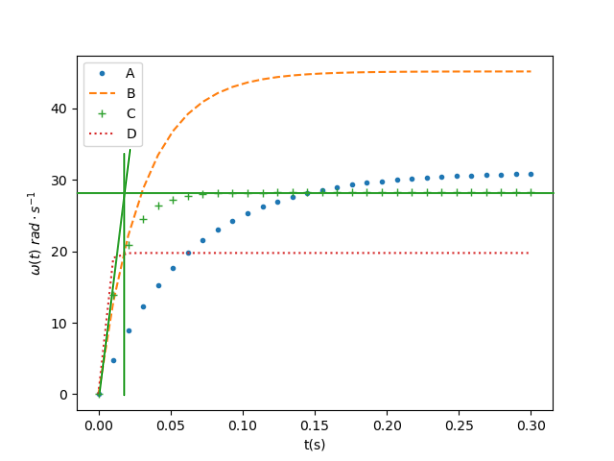
\includegraphics[width=.7\linewidth]{img/fig02_cor}
\end{center}
}

\reponse{4}{}{$T_{R5\%}=3\cdot\tau=3\cdot 17=51ms$.}

\reponse{3}{}{La vitesse de translation de la porte peut s'écrire comme la vitesse de rotation du moteur multipliée par le rayon de la roue car il s'agit d'une transmission poulie courroie.}

\reponse{4}{}{
\[
v_{p+\infty} = r\cdot\omega_\infty = 0.02 \times 30
\]

\[
v_\infty \approx 0.6\ m\cdot s^{-1}
\]}

\reponse{3}{}{
La porte parcours $1.2m$ à la vitesse de $0.6m\cdot s^{-1}$, cela correspond à une durée de fermeture $T=\dfrac{1.2}{0.6}=2s$.
}

\reponse{5}{}{
\[\Delta=\left(\dfrac{2\cdot\xi}{\omega_0}\right)^2-\dfrac{4}{\omega_0^2}\]

\[p=\dfrac{-\dfrac{2\cdot\xi}{\omega_0}\pm\sqrt{\Delta}}{\dfrac{2}{\omega_0^2}}=-\omega_0\cdot\left(\xi\pm\cdot\sqrt{\xi^2-1}\right)\]
}

\reponse{4}{}{
$\Delta=0.3^2-4\cdot 0.02=0.09-0.04=0.01$

$p=\dfrac{-0.3\pm\sqrt{0.01}}{2\cdot 0.02}$

$p=\dfrac{-0.3\pm 0.1}{0.04}$

$p_1=-5$ et $p_2=-10$

$\tau_1=\dfrac{1}{5}=0.2s$ et $\tau_2=\dfrac{1}{10}=0.1s$


\[H_3(p)=\dfrac{8}{(1+0.2\cdot p)\cdot (1+0.1\cdot p)}\]
}

\reponse{10}{}{
\[S_3(p)=\dfrac{8\cdot 7}{p\cdot (1+\tau_1\cdot p)\cdot (1+\tau_2\cdot p)}\]

\[S_3(p)=\dfrac{A\cdot (1+\tau_1\cdot p)\cdot (1+\tau_2\cdot p)+B\cdot p\cdot (1+\tau_2\cdot p)+C\cdot p\cdot (1+\tau_1\cdot p)}{p\cdot (1+\tau_1\cdot p)\cdot (1+\tau_2\cdot p)}\]

\[S_3(p)=\dfrac{A +(A\cdot \tau_1+A\cdot \tau_2+B+C)\cdot p+(A\cdot\tau_1\cdot\tau_2+B\cdot\tau_2+C\cdot\tau_1)\cdot p^2}{p\cdot (1+\tau_1\cdot p)\cdot (1+\tau_2\cdot p)}\]

Ainsi:
\begin{eqnarray}
A=8\\
A\cdot \tau_1+A\cdot \tau_2+B+C=0\\
A\cdot\tau_1\cdot\tau_2+B\cdot\tau_2+C\cdot\tau_1=0
\end{eqnarray}

Calcul : $\tau_1\cdot Eq4 -Eq5$

$A\cdot \tau_1^2+B\cdot (\tau_1-\tau_2)=0$

$B=-\dfrac{A\cdot \tau_1^2}{\tau_1-\tau_2}$

De même avec le calcul : $\tau_2\cdot Eq4 -Eq5$

$C=-\dfrac{A\cdot \tau_2^2}{\tau_1-\tau_2}$

$A=56$

$B=-\dfrac{56\cdot 0.2^2}{0.2-0.1}=-\dfrac{7\cdot 0.32}{0.1}=-22.4$

$C=-\dfrac{56\cdot 0.1^2}{0.1-0.2}=\dfrac{56\cdot 0.1^2}{0.1}=5.6$

}

\end{document}
